\documentclass[11pt,a4paper,oneside]{article}
\usepackage[hangul]{kotex}
\usepackage{olymp}
\usepackage{graphicx}
\usepackage{subcaption}
\usepackage{enumitem}
\usepackage{amsmath}
\usepackage[english]{babel}
\usepackage{amssymb}
\usepackage{import}
\usepackage{multirow}
\usepackage{xcolor}
\usepackage{minted}

% 키파: XeLaTeX 혹은 LuaLaTeX로 컴파일한 뒤 아래 두 줄을 주석해제하면 오류 없이 얼추 비슷한 결과를 얻습니다. 오류 확인을 원할 때 사용하세요.
\usepackage{fontspec}
\setmainhangulfont{NanumMyeongjo}

\usepackage{tikz}
\usepackage{pdfpages}


\definecolor{boj}{RGB}{0,118,191}
\definecolor{ucpc-orange}{RGB}{255,153,0}
\definecolor{acgreen}{RGB}{0,159,107}
\definecolor{wared}{RGB}{231,76,60}

\definecolor{acbronze}{RGB}{173,86,0}
\definecolor{acsilver}{RGB}{67,95,122}
\definecolor{acgold}{RGB}{236,154,0}
\definecolor{acplatinum}{RGB}{39,226,164}
\definecolor{acdiamond}{RGB}{0,180,252}
\definecolor{acruby}{RGB}{255,0,98}

\renewcommand{\baselinestretch}{1.0}

\contest{2026 Soongsil Programming Contest}{SCCC@SoongsilU}{May 23th, 2026}

\begin{document}
    \def\NoInputFileName{}
    \def\NoOutputFileName{}
    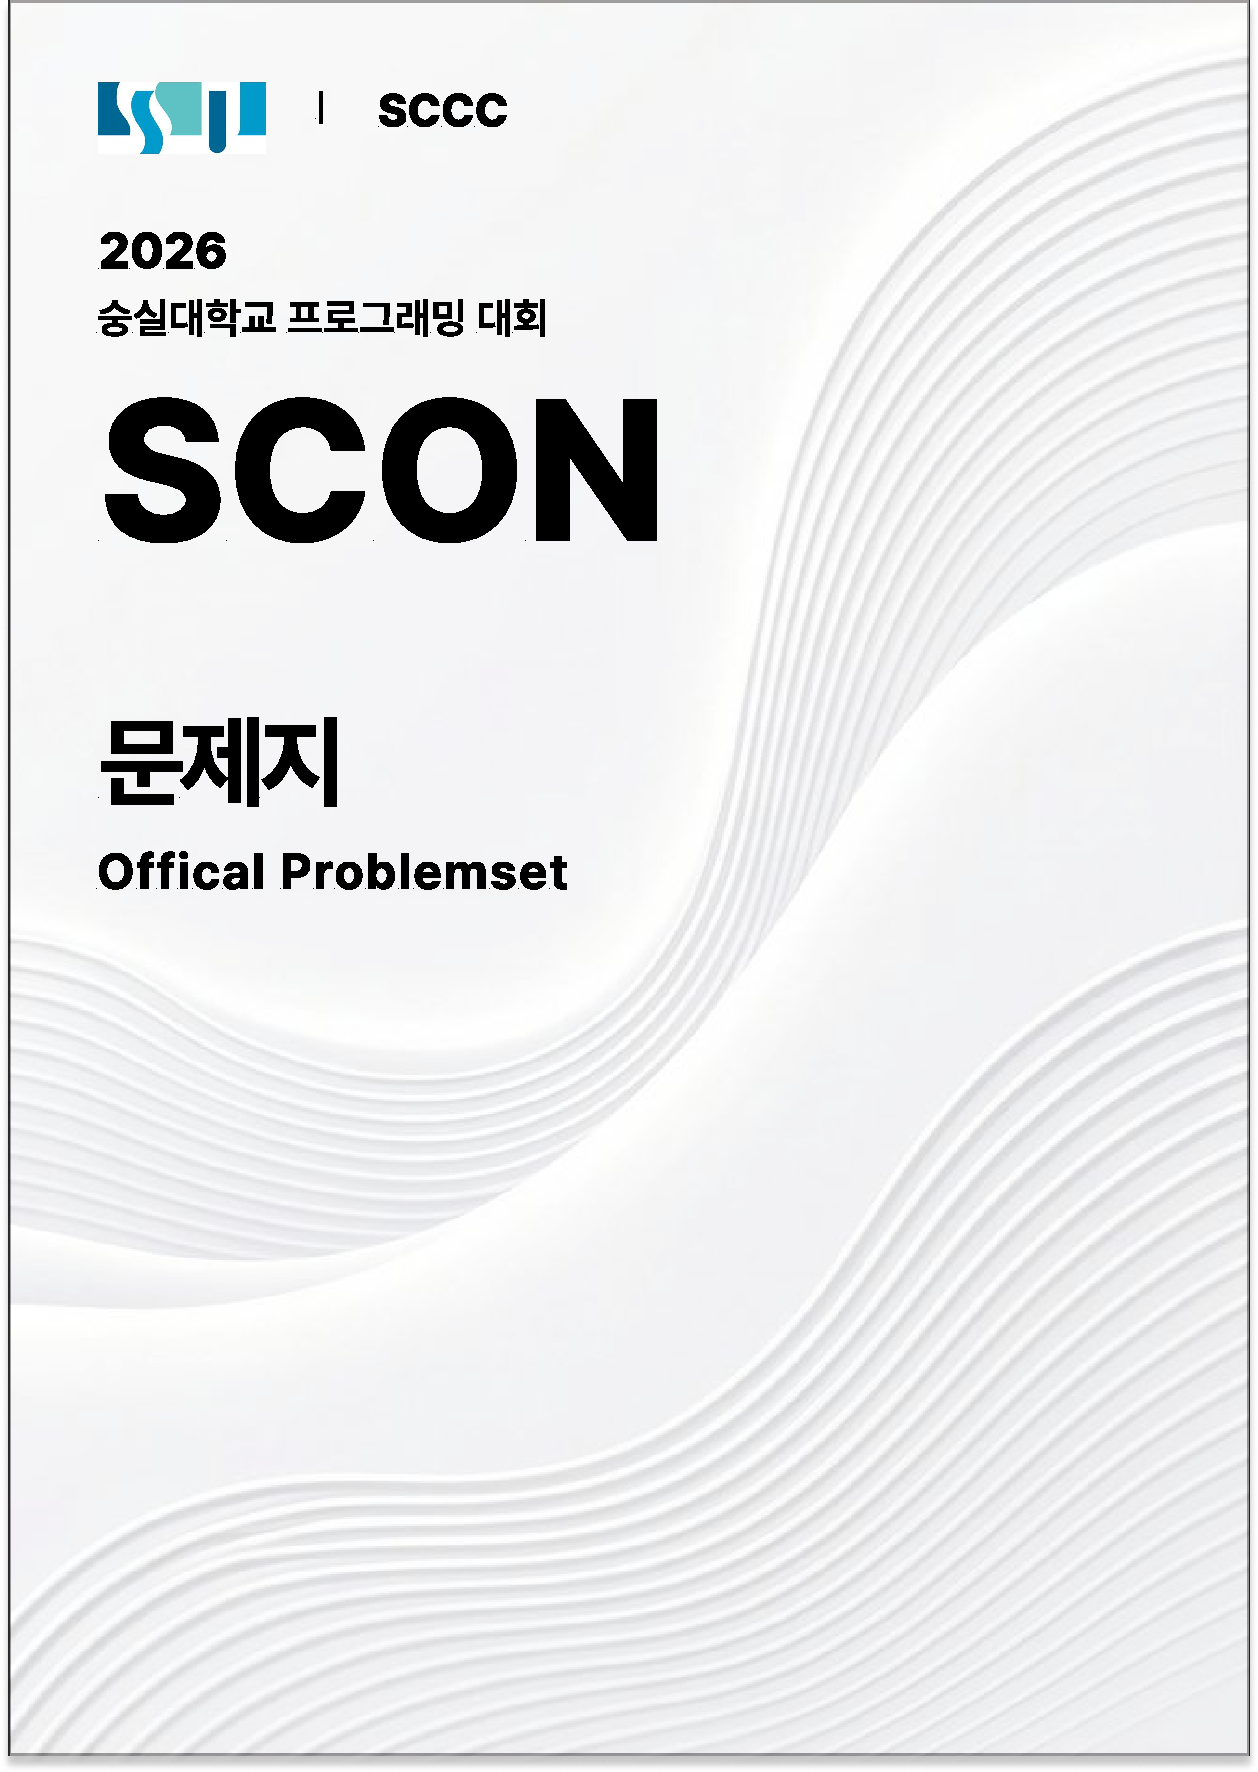
\includepdf[pages=1,offset=25mm -38mm]{cover-2026scon.pdf}
%
    \import{./}{language.tex} \pagebreak
    \import{./}{rule.tex} \pagebreak
%
    \begin{center}
    
    \vspace*{15mm}
    {
        \Huge
        \textbf{2026 Soongsil Programming Contest}
        
        \vspace{25mm}
        Problem List
        \vspace{10mm}
    }
    
    \begin{tabular}{|c|l|r|r|r|}
    \hline
    \# & Problem Name & Time limit & Memory limit & Page \\ \hline
        A & Where is my ``ICP" & 1 second\phantom{s} & 1024MiB & \phantom{0}8 -- \phantom{0}9 \\ \hline
        B & 숭실대입구역 & 1 seconds & 1024MiB & 10 -- 10 \\ \hline
        C & 크림 먼저, 잼 먼저 & 1 second\phantom{s} & 1024MiB & 11 -- 12 \\ \hline
        D & 사전순 최소 & 1 second\phantom{s} & 1024MiB & 13 -- 14 \\ \hline
        E & 구간 뒤집기 & 1 second\phantom{s} & 1024MiB & 15 -- 15 \\ \hline
        F & 덜 개성있는 구간 & 1 second\phantom{s} & 1024MiB & 16 -- 16 \\ \hline
        G & 보안 & 1 second\phantom{s} & 1024MiB & 17 -- 18 \\ \hline
        H & 같게 만들기 & 1 second\phantom{s} & 1024MiB & 19 -- 20 \\ \hline
        I & 분탕의 신 & 1 second\phantom{s} & 1024MiB & 21 -- 23 \\ \hline
        J & SCON 마법진 & 1 seconds & 1024MiB & 24 -- 26 \\ \hline
        K & XOR 팰린드롬 & 2 seconds & 1024MiB & 27 -- 28 \\ \hline
        L & 뱀 수열 & 3 seconds & 1024MiB & 29 -- 30 \\ \hline
    \end{tabular}

    \vspace{5mm}
    
    문제지에 있는 문제가 총 12문제가 맞는지 확인하시길 바랍니다.

    문제는 출제진이 생각하는 난이도순으로 정렬되어 있지만, 모든 문제를 읽고 고민하는 것을 권장합니다.

    모든 문제는 C++17, Java 15, PyPy3으로 풀 수 있음을 보장합니다. (단, Python 3는 보장하지 않음)
    
    \end{center}
    	
    \pagebreak
    
    \import{2026/where-is-my-icp/}{main.tex} \pagebreak
    \import{2026/station/}{main.tex} \pagebreak
    \import{2026/cream-jam/}{main.tex} \pagebreak
    \import{2026/lexi/}{main.tex} \pagebreak
    \import{2026/flip/}{main.tex} \pagebreak
    \import{2026/unique/}{main.tex} \pagebreak
    \import{2026/protect/}{main.tex} \pagebreak
    \import{2026/same/}{main.tex} \pagebreak
    \import{2026/god/}{main.tex} \pagebreak
    \import{2026/scon-magic-graph/}{main.tex} \pagebreak
    \import{2026/xor/}{main.tex} \pagebreak
    \import{2026/snake-seq/}{main.tex} \pagebreak



    % \begingroup
    %     \makeatletter
    %     \setcounter{problem}{0}
        
    %     \let\OldAlph\Alph
    %     \renewcommand{\Alph}[1]{P\OldAlph{#1}}
        
    %     \import{2026/PSpoker/}{main.tex} \pagebreak
    %     \import{2026/unique-origin/}{main.tex} \pagebreak
    %     \import{2026/SC_ON/}{main.tex} \pagebreak
        
    %     \makeatother
    % \endgroup
    
    
\end{document}